% Chapter 3

\chapter{Použité metódy merania štruktúry MOS.}\label{Chapter3}
\lhead{Kapitola 3. \emph{Použité metódy merania štruktúry MOS}}
%- - - - - - - - - - - - - - - - - - - - - - - - - - - - - - - - - - -

Kapacitne-napäťové (C-V) metódy, ktorými sa v tejto práci budeme
zaoberať, poskytujú komplexné informácie o elektro-fyzikálnych
parametroch štruktúry MOS\@. Pre určenie niektorých parametrov
postačuje vyhodnotenie dát nameraných pomocou jednej metódy, no vo
väčšine prípadov kombináciou viacerých metód možno získať presnejšie
výsledky.  V predchádzajúcej kapitole sme na príklade výpočtu C-V
závislosti ideálnej štruktúry MOS demonštrovali rozdiely medzi
napäťovými závislosťami kapacity štruktúry MOS, meranými rozličnými
metódami:

\begin{itemize}
\item nízkofrekvenčnou (prípadne kvázistatickou) C-V metódou
\item rovnovážnou vysokofrekvenčnou C-V metódou
\item nerovnovážnou vysokofrekvenčnou C-V metódou.
\end{itemize}

Okrem uvedených metód sme v dizertačnej práci použili Q-C metódu,
ktorá kombinuje vlastnosti vysokofrekvenčnej a nízkofrekvenčnej C-V
metódy. Určenie tých istých C-V závislostí pomocou rôznych metód
zároveň predstavuje určitý druh kontroly presnosti merania.  To je
výhodné hlavne v prípadoch, kedy určenie absolútnej chyby merania
predstavuje komplexný problém. Pre meranie generačného času života
minoritných nosičov náboja sme použili metódu konštantnej šírky
OPN~\cite{3.1}, ktorej výhodou oproti klasickej Zerbstovej C-t
metóde~\cite{3.2} je väčšia rýchlosť merania. Modifikácia metódy
konštantnej šírky OPN~\cite{3.3} zároveň eliminuje vplyv bočnej
injekcie minoritných nosičov náboja do OPN zo substrátu.

Výhodou uvedených metód je, že nie sú deštruktívne, čo ich v spojení s
ich rýchlosťou predurčuje pre rutinné použitie v priemysle.  V
laboratórnych podmienkach je vhodné tieto metódy overiť pomocou
ďalších metód, ktoré možno považovať za doplnkové. Tak je tomu pri
meraní koncentračného profilu prímesí, napríklad metódou rozptylového
odporu, elektrochemickou kapacitnou metódou, prípadne SIMS\@. Vhodné
je aj overenie koncentračného profilu pomocou simulácie
technologického procesu. Pri skúmaní energetických stavov
nachádzajúcich sa v zakázanom pásme polovodiča, kvalitné informácie
poskytuje metóda DLTS\@.

Uvedené C-V metódy predstavujú podmnožinu širokej oblasti diagnostiky
štruktúr MOS pomocou kapacitných meraní.  Následujúca schéma
znázorňuje ich vzťah ku skúmaným parametrom, ktoré boli predmetom
tejto práce a zároveň poukazuje na okruhy problémov, ktoré bolo
potrebné riešiť.

\begin{diagram}
  \centering
  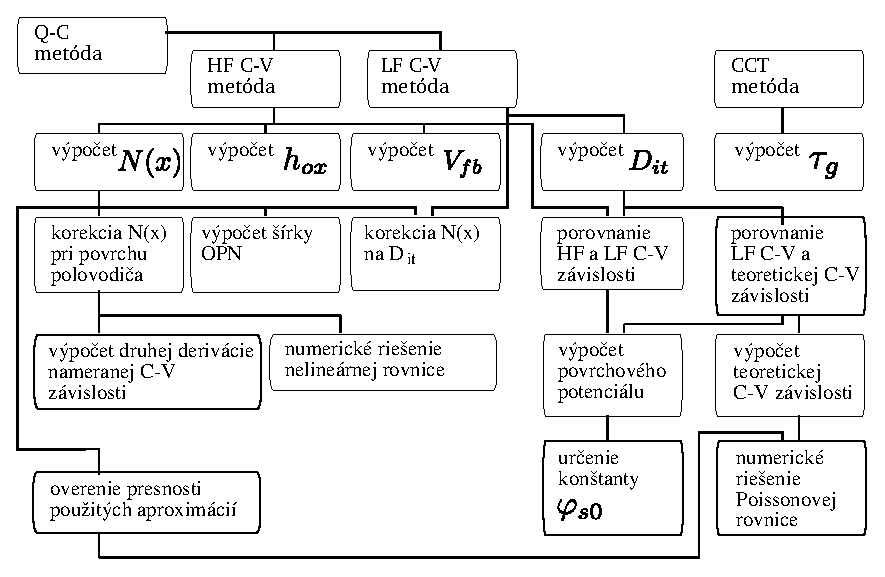
\includegraphics[width=\textwidth,height=\textheight,scale=0.7,keepaspectratio]{Figures/diagram-1.EPS}\label{diagram:1}
\end{diagram}

\section{Vysokofrekvenčná C-V metóda.}\label{sec:3.1}

Pri meraní vysokofrekvenčnou kapacitnou metódou je MOS štruktúra
jednosmerným hradlovým napätím privedená do požadovaného stavu a jej
kapacita sa určí z prúdovej odozvy na vysokofrekvenčný signál malej
amplitúdy, ktorý je nasuperponovaný na jednosmerné hradlové
napätie. Meraním fázového posuvu medzi vysokofrekvenčným napäťovým
signálom a prúdom možno okrem kapacity zároveň vyhodnotiť aj vodivosť
štruktúry. Veľkosť frekvencie meracieho signálu je daná kompromisom
medzi požiadavkou čo najvyššej frekvencie zo strany ovplyvnenia
merania rýchlymi pascami rozhrania $Si-SiO_2$ a technickými možnosťami
štandardných meracích prístrojov.  V našom experimente sme použili
prístroj HP4280a, ktorého merací signál má pevne stanovenú frekvenciu
1 MHz a veľkosť amplitúdy meracieho signálu možno voliť 10 mV, alebo
30 mV.  Spomenutý prístroj možno riadiť pomocou zbernice IMS-2. Treba
uviesť, že prístroj v spojení s riadiacim počítacom PC AT je schopný v
blokovom prenose zmerať a v binárnom formáte preniesť do riadiaceho
počítača 680 bodov (čo je limit pre blokový prenos) C-V a G-V
závislosti za 25 sekúnd.  Uvedený časový údaj uvádzame na základe
vykonaných vlastných experimentov.

\section{Kvázistatická C-V metóda.}\label{sec:3.2}

Pri meraní kvázistatickou kapacitnou metódou je MOS štruktúra nabíjaná
pomalým, v čase narastajúcim hradlovým napätím. Kapacita MOS štruktúry
je určená ako závislosť nabíjacieho prúdu a rýchlosti nárastu
hradlového napätia.  Z uvedeného vyplýva, že na realizáciu metódy je
potrebný zdroj kontinuálne narastajúceho napätia a
ampérmeter. Rýchlosť narastania napätia musí byť dostatočne malá, aby
bola štruktúra počas merania stále v termodynamickej rovnováhe. Na
druhej strane zase so zmenšovaním rýchlosti sa zmenšuje aj prúd, ktorý
musíme merať. Pre väčšinu meraných vzoriek vyhovovala rýchlosť rádove
$10^{-2}V/s$, čo predstavuje pre kapacitu $100pF$ nabíjací prúd
$10^{-12}A$. V našom experimente sme použili na meranie prúdu
elektrometer Keithley 642, ktorý meria prúd v rozsahu od $10^{-8}A$ do
$10^{-17}A$ s rozlíšením 5 číslic na rozsah.  Treba podotknúť, že
okrem iných vynikajúcich vlastností prístroja výrobca zaručuje
efektívnu hodnotu šumu menšiu ako $8\times10^{-17}A$. Zdroj
narastajúceho napätia, ktorý bol postavený na našej katedre, umožňuje
nastavenie rýchlosti nárastu napätia v rozsahoch od $10V/s$ do
$10^{-3}V/s$ s rozlíšením 1\% rozsahu. Oba prístroje možno riadiť
pomocou zbernice IMS-2.  Hlavným zdrojom chýb pri kvázistatickej
metóde je nepresnosť určenia rýchlosti nárastu napätia
hradla~\cite{1.5}. Pred každým meraním je potrebné presne zmerať
rýchlosť nárastu napätia, ktorá sa potom použije pri výpočte
kapacity. Rýchlosť nárastu napätia pre zvolený rozsah určujeme v našom
prípade z podielu zmeny napätia a času za 10 s.  Uvedená hodnota má
potom význam strednej hodnoty a jej použitie pri výpočte predpokladá
lineárny nárast napätia, ktorý sme experimentálne overili pre
reprezentatívnu vzorku rozsahov nárastu napätia v čase.

\section{Q-C metóda.}\label{sec:3.3}

Q-C metóda~\cite{3.4} predstavuje kombináciu vysokofrekvenčnej C-V
metódy a nábojovej Q-V metódy~\cite{3.5}. Jej princíp je následovný. Do
série s kondenzátorom tvoreným štruktúrou MOS je zapojená napäťovo
nezávislá kapacita, ktorú označíme $C_i$. Na sériovo-paralelné
zapojenie kondenzátorov, ktoré je znázornené na obrázku~\ref{fig:3.1},
pripojíme jednosmerné napätie $V_a$ a meriame napätie $V_i$ v
spoločnom bode zapojenia kondenzátorov, ktoré predstavujú kapacitný
delič. Kondenzátory označené $C_w$ a $C_x$ znázorňujú parazitné
kapacity. $C_w$ je kapacita medzi stolíkom a zdvihnutým hrotom sondy a
$C_x$ je kapacita spoločného bodu zapojenia kondenzátorov voči
zemi. Zároveň s meraním napätia $V_i$ zmeriame aj kapacitu $C_m$ a
vodivosť $G_m$ pomocou vysokofrekvenčného signálu nasuperponovaného na
napätí $V_a$.

\begin{figure}[h!]\centering
  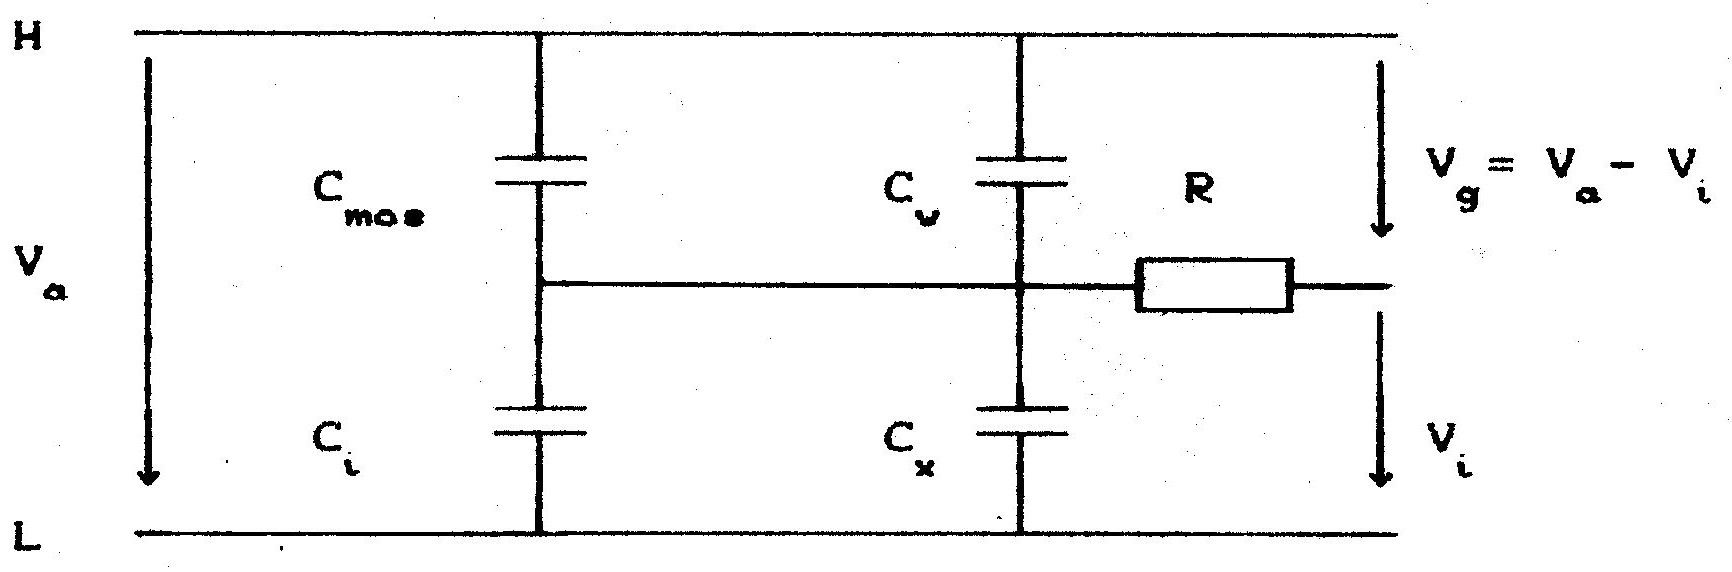
\includegraphics{Figures/fig-3-1.eps}% chktex-file 8
  \caption[Schematické znázornenie zapojenia kondenzátorov Q-C 
metódy]{Schematické znázornenie zapojenia kondenzátorov Q-C 
metódy}\label{fig:3.1}
\end{figure}

Medzi spoločný bod zapojenia kondenzátorov a vstup voltmetra je
pripojený odpor, ktorý spolu s kapacitou prívodných vodičov voltmetra
a vstupnou kapacitou voltmetra tvorí dolnopriepustný filter,
spôsobujúci, že merané napätie nie je ovplyvnené vysokofrekvenčným
signálom. Z uvedeného zároveň vyplýva, že veľkosť kapacity medzi
spoločným bodom zapojenia a bodom L sa bude líšiť pre jednosmerné a
vysokofrekvenčné meranie. Označme preto kapacitu $C_i$ pre jednosmerné
meranie $C_{iLF}$ a pre vysokofrekvenčné meranie $C_{iHF}$.  Spomenutý
odpor spolu so vstupným odporom voltmetra tvorí napäťový delič.  Aby
tým nebolo ovplyvnené meranie napätia, treba použiť voltmeter s
vysokým vstupným odporom.  Tu treba spomenúť vhodnosť použitia
elektromeru Keithley 642, ktorého vstupný odpor v režime merania
napätia je približne $10^{16} \Omega$ a jeho parazitná vstupná
kapacita sú $2 pF$. Detailný popis zapojenia Q-C metódy, eliminácia
parazitných kapacít, prípadne metodika ich merania je popísaná v
dodatku~\ref{app:AppendixE}. Ak poznáme kapacitu oxidovej vrstvy
štruktúry MOS $C_{ox}$ a veľkosť kapacity $C_{iLF}$, môžeme vypočítať
hodnotu povrchového potenciálu $\varphi_s$ z nasledovného vzťahu,
odvodeného v dodatku~\ref{app:AppendixF}.

\begin{equation}
  \varphi_s = \varphi_{s0} + V_g ( 1 + \frac{C_w}{C_{ox}}) - V_i \frac{C_{iLF}+C_x}{C_{ox}}
  \label{eq:3.1}
\end{equation}

Zároveň môžeme určiť nízkofrekvenčnú kapacitu štruktúry MOS

\begin{equation}
  C^{LF}_{mos} = C_{ox} (1 - \frac{d\varphi_s}{dV_g})
  \label{eq:3.2}
\end{equation}

Poruchové náboje nachádzajúce sa v meranej štruktúre MOS spôsobujú, že
povrchový potenciál polovodiča nadobúda hodnotu $\varphi_{s0}$ aj pri
nulovom napätí hradla. Veľkosť tejto konštanty možno určiť z
porovnania nameranej a teoretickej závislosti povrchového potenciálu
od šírky OPN $\varphi(x)$.  Metóda určenia $\varphi_{s0}$ je popísaná
v dodatku~\ref{app:AppendixG}. Tu možno poznamenať, že pre výpočet
$C^{LF}_{mos}$ hodnotu tejto konštanty nepotrebujeme, ako je zrejmé zo
vzťahov~\ref{eq:3.1} a~\ref{eq:3.2}.

Z nameraných hodnôt $C_m$ a $G_m$ môžeme určiť vysokofrekvenčnú
kapacitu štruktúry MOS pomocou nasledovných vzťahov.  Najprv
vypočítame odpovedajúci odpor $R_m$ a reaktanciu $X_m$

\begin{subequations}\label{eq:3.3}
  \begin{align}
    R_m &= \frac{G_m}{G^2_m + {(\omega C_m)}^2}\label{eq:3.3a}\\[0.3cm]
    X_m &= \frac{\omega C_m}{G^2_m + {(\omega C_m)}^2}\label{eq:3.3b}\\[0.3cm]
    \intertext{,ktoré použijeme vo vzťahu}
    C^{HF}_{mos} &= - \cfrac{R^2_m + {(X_m + \frac{1}{\omega C_{iHF}} + \omega C_w D^2)}^2}{\omega D^2{(X_m + \frac{1}{\omega C_{iHF}} + \omega C_{w} D^2)}^2}\label{eq:3.3c}\\[0.3cm]
    \intertext{,kde}
    D^2 &= R^2_m + {(X_m + \frac{1}{\omega C_{iHF}})}^2\label{eq:3.3d}
  \end{align}
\end{subequations}

Podrobný popis a odvodenie uvedených vzťahov sú popísané v
dodatku~\ref{app:AppendixE}. Q-C metóda poskytuje celý rad výhod.
Umožňuje simultánne meranie vysokofrekvenčnej a nízkofrekvenčnej C-V
závislosti, čo zaručuje rovnaké podmienky merania pre obe závislosti a
vylučuje možnosť ich vzájomného napäťového posuvu, ktorý sa môže
objaviť ak by boli závislosti snímané sekvenčne. Zároveň meranie
nízkofrekvenčnej C-V závislosti je statické a nie je závisle od
dynamiky hradlového napätia.

Pre určenie koncentračného profilu prímesí v podpovrchovej oblasti
polovodiča je výhodné poznať priebeh povrchového potenciálu, čo
umožňuje výpočet nezaťažený pascami rozhrania $Si-SiO_2$. Uvedené
výhody sú vykompenzované náročnosťou metódy na použité prístroje.
Kritickým bodom realizácie metódy je odizolovanie spoločného bodu
zapojenia kondenzátorov. Pripojené napätie $V_a$ sa musí rozložiť na
kondenzátoroch podľa ich kapacít a nie podľa ich zvodových odporov.
To vyžaduje použitie kvalitného kondenzátora $C_i$ a usporiadanie
rozloženia jednotlivých komponentov metódy tak, aby bol zvodový prúd
zo spoločného bodu na zem čo najmenší. Tým sú z použitia Q-C metódy
vylúčené štruktúry MOS, ktoré majú veľké zvodové prúdy spôsobené
nedokonalosťou oxidovej vrstvy. Pre meranie v stave termodynamickej
rovnováhy, ako uvádzajú autori metódy~\cite{3.7}, je potrebné aby sa
napätie $V_i$ nemenilo najmenej počas 10 sekúnd o veľkosť rádove
$10^{-3}V$. Pre účely určenia koncentračného profilu môžeme merať
nerovnovážnu C-V závislosť, pri ktorej sa zvodové prúdy zo spoločného
bodu na zem neprejavia v takej miere, pretože merané napätie je
odčítavané okamžite po priložení napätia. Na obrázku~\ref{fig:3.2} sú
znázornené normované priebehy HF C-V závislosti štruktúry MOS a
priebehu povrchového potenciálu od napätia hradla určené pomocou Q-C
metódy pre meranie v stave termodynamickej rovnováhy a v stave
hlbokého ochudobnenia. Použité prístroje v implementácii metódy na
našom oddelení~\cite{3.8,3.9} možno riadiť pomocou zbernice IMS-2 a
namerané hodnoty napätí $V_a$, $V_i$, kapacity $C_m$ a vodivosti $G_m$
uložiť do diskového súboru pre ďalšie spracovanie.

\begin{figure}[h!]\centering
  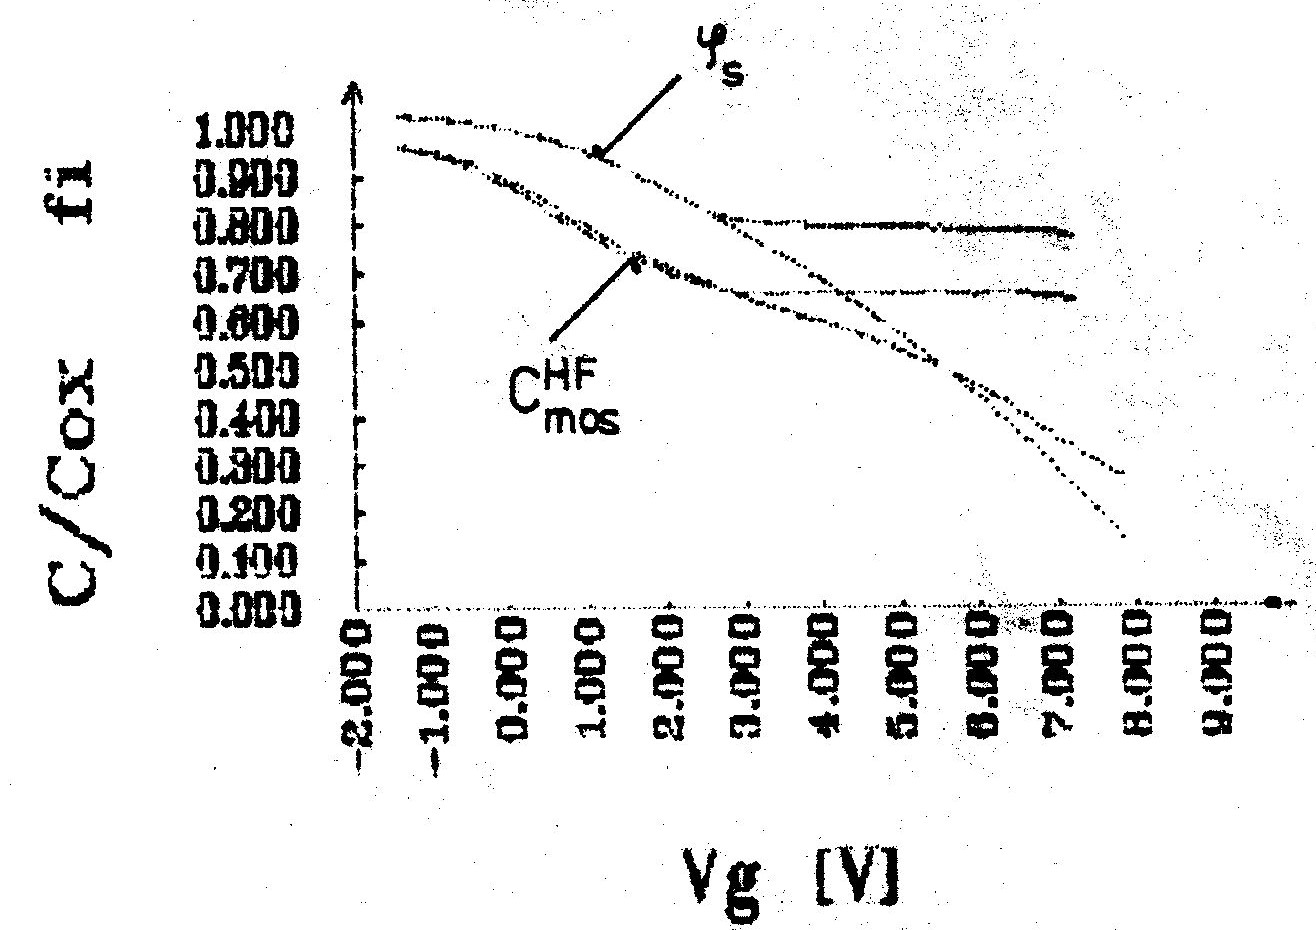
\includegraphics{Figures/fig-3-2.eps}
  \caption[Normované priebehy HF C-V závislosti štruktúry MOS a priebehu
  povrchového potenciálu od napätia hradla určené pomocou Q-C metódy
  pre meranie v stave termodynamickej rovnováhy a v stave hlbokého
  ochudobnenia]{Normované priebehy HF C-V závislosti štruktúry
  MOS a priebehu povrchového potenciálu od napätia hradla určené
  pomocou Q-C metódy pre meranie v stave termodynamickej rovnováhy a v
  stave hlbokého ochudobnenia. Priebehy $\varphi_s(V_g)$ sú zobrazené
  s použitím normovania $1 - \frac{\varphi_s}{\varphi_{norm}}$, kde
  $\varphi_{norm}=3.33V$.}\label{fig:3.2}
\end{figure}
%OBR7.BIT

Pre overenie presnosti Q-C metódy sme na tej istej štruktúre MOS
urobili samostatné vysokofrekvenčné a nízkofrekvenčné meranie a
zároveň vypočítali tie isté kapacitné závislosti z nameraných hodnôt
Q-C metódy.  Výsledné krivky sú na obrázkoch~\ref{fig:3.3} a~\ref{fig:3.4}.

Pre kvantitatívne porovnanie výsledkov znázornených na
obrázku~\ref{fig:3.3} a~\ref{fig:3.4} uvádzame v tabuľke~\ref{tab:3.1}
a~\ref{tab:3.2} číselné hodnoty normovaných kapacít $C^{HF}_{mos}$ a
$C^{LF}_{mos}$ pre metódy HF, LF a Q-C a ich rozdiel vyjadrený
relatívnou chybou. Z tabuliek vidieť rozdiel medzi jednotlivými C-V
závislosťami, čo je spôsobené jednak nepresnosťami pri určovaní
parazitných kapacít a jednak zvodovými prúdmi použitých
kondenzátorov. Autori metódy doporučujú pre elimináciu zvodových
prúdov, ktoré spôsobuje vlhkosť prostredia, použiť vzduchový
kondenzátor $C_i$ a na meranú vzorku usmerniť v priebehu merania prúd
dusíka, ktorý zabráni kondenzovaniu vodných pár z okolia.

\newpage
\begin{figure}[h!]\centering
  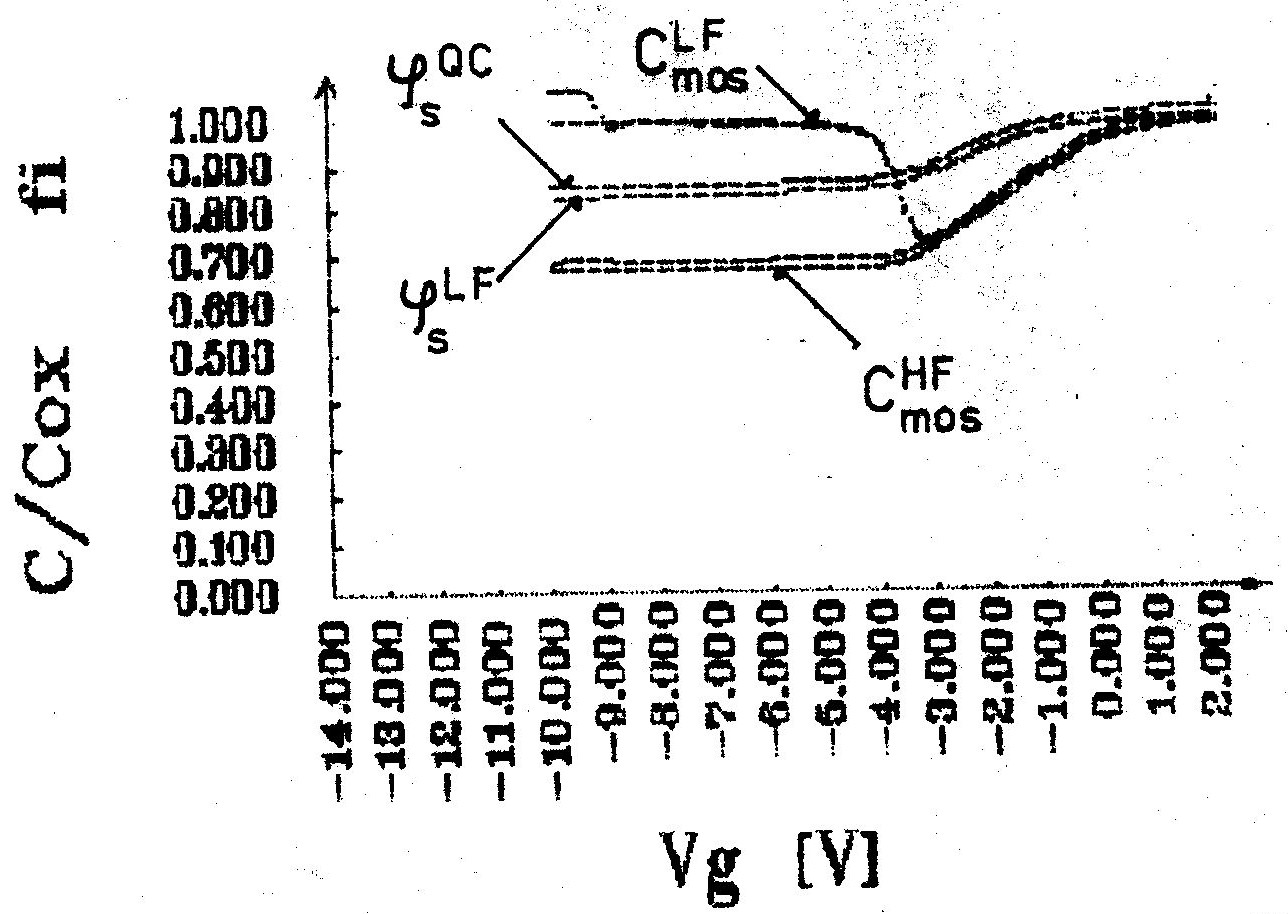
\includegraphics{Figures/fig-3-3.eps}
  \caption[Normované priebehy kapacity štruktúry MOS so substrátom typu
  N ako funkcie napätia hradla pre rovnovážne vysokofrekvenčné a
  kvázistatické meranie]{Normované priebehy kapacity štruktúry MOS so
  substrátom typu N ako funkcie napätia hradla pre rovnovážne
  vysokofrekvenčné a kvázistatické meranie.  Zároveň sú znázornené tie
  isté charakteristiky získané pomocou Q-C metódy. Pre úplnosť je na
  obrázku znázornená závislosť povrchového potenciálu
  ${\varphi_s(V_g)}^{QC}$ získaná pomocou Q-C metódy a závislosť
  ${\varphi_s(V_g)}^{LF}$ vypočítaná integrovaním nízkofrekvenčnej C-V
  závislosti pomocou Berglundovho integrálu.  Priebehy
  $\varphi_s(V_g)$ sú zobrazené s použitím normovania $1 -
  \frac{\varphi_s}{\varphi_{norm}}$, kde $\varphi_{norm}=-3.33V$.}\label{fig:3.3}
\end{figure}
%OBR5.BIT

\begin{table}[h!]\centering
  \begin{tabular}{c c c c c c}
    \multicolumn{3}{l}{$C^{HF}_{mos}$} & \multicolumn{3}{l}{$C^{LF}_{mos}$} \\
    HF[\%] & QC[\%] & $\Delta_r$[\%] & LF[\%] & QC[\%] & $\Delta_r$[\%] \\
    \hline% chktex-file 44
    99.67 & 98.30 & +1.37 & 97.85 & 99.14 & -1.32 \\
    98.56 & 96.69 & +1.89 & 96.59 & 97.05 & -0.47 \\
    98.56 & 96.69 & +1.89 & 96.59 & 97.05 & -0.47 \\
    95.73 & 93.89 & +1.92 & 93.93 & 94.51 & -0.61 \\
    89.89 & 87.75 & +2.39 & 88.26 & 88.57 & -0.36 \\
    82.15 & 80.17 & +2.41 & 81.43 & 81.82 & -0.47 \\
    74.83 & 73.09 & +2.33 & 73.79 & 74.57 & -1.06 \\
    69.69 & 67.81 & +2.70 & 86.08 & 86.33 & -0.29 \\
    69.10 & 67.20 & +2.74 & 97.20 & 97.73 & -0.54 \\
    68.97 & 67.08 & +2.74 & 98.27 & 98.74 & -0.48 \\
    68.91 & 67.03 & +2.72 & 98.75 & 99.38 & -0.64 \\
    68.90 & 67.01 & +2.75 & 99.04 & 98.68 & -0.36 \\
    68.90 & 67.03 & +2.70 & 99.20 & 99.87 & -0.67 \\
  \end{tabular}
  \caption[Porovnanie normovanej vysokofrekvenčnej a nízkofrekvenčnej
    kapacity štruktúry MOS (obrázok~\ref{fig:3.3}) pre metódy HF, LF a
    Q-C]{Porovnanie normovanej vysokofrekvenčnej a nízkofrekvenčnej
    kapacity štruktúry MOS (obrázok~\ref{fig:3.3}) pre metódy HF, LF a
    Q-C. Rozdiel kriviek je vyjadrený relatívnou chybou.}\label{tab:3.1}
\end{table}

\newpage
\begin{figure}[h!]\centering
  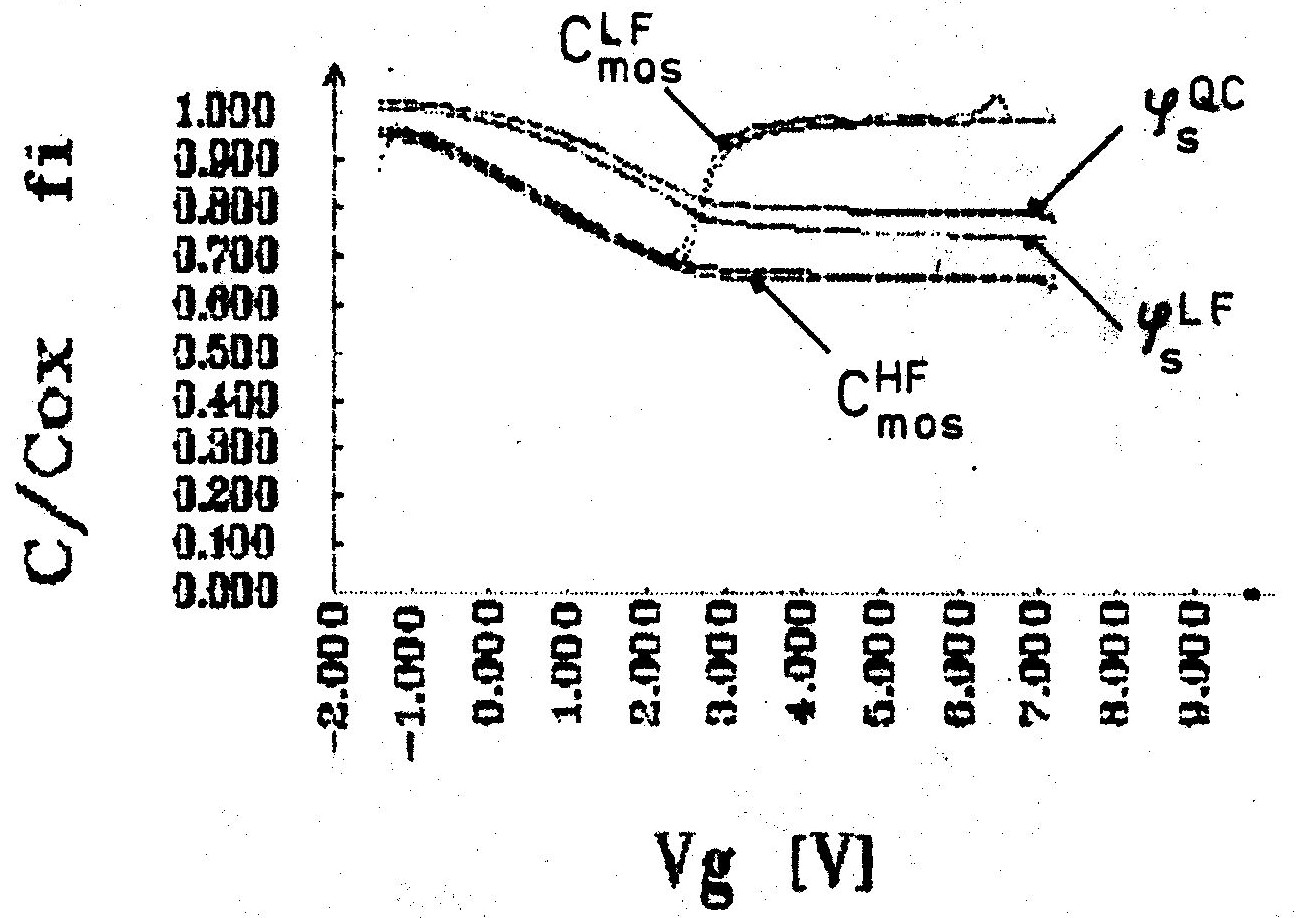
\includegraphics{Figures/fig-3-4.eps}
  \caption[Normované priebehy kapacity štruktúry MOS so substrátom typu
  P ako funkcie napätia hradla pre rovnovážne vysokofrekvenčné a
  kvázistatické meranie]{Normované priebehy kapacity štruktúry MOS so
  substrátom typu P ako funkcie napätia hradla pre rovnovážne
  vysokofrekvenčné a kvázistatické meranie.  Zároveň sú znázornené tie
  isté charakteristiky získané pomocou Q-C metódy. Pre úplnosť je na
  obrázku znázornená závislosť povrchového potenciálu
  ${\varphi_s(V_g)}^{QC}$ získaná pomocou Q-C metódy a závislosť
  ${\varphi_s(V_g)}^{LF}$ vypočítaná integrovaním nízkofrekvenčnej C-V
  závislosti pomocou Berglundovho integrálu.  Priebehy
  $\varphi_s(V_g)$ sú zobrazené s použitím normovania $1 -
  \frac{\varphi_s}{\varphi_{norm}}$, kde $\varphi_{norm}=3.33V$.}\label{fig:3.4}
\end{figure}
%OBR6.BIT

\begin{table}[h!]\centering
  \begin{tabular}{c c c c c c}
  \multicolumn{3}{l}{$C^{HF}_{mos}$} & \multicolumn{3}{l}{$C^{LF}_{mos}$} \\
  HF[\%] & QC[\%] & $\Delta_r$[\%] & LF[\%] & QC[\%] & $\Delta_r$[\%] \\
  \hline
  96.30 & 95.71 & +0.62 & 94.80 & 94.89 & -0.09 \\
  92.88 & 92.07 & +0.87 & 91.03 & 92.83 & -1.98 \\
  87.52 & 86.48 & +1.19 & 85.97 & 87.53 & -1.81 \\
  81.39 & 80.09 & +1.60 & 79.70 & 81.20 & -1.88 \\
  75.71 & 74.55 & +1.53 & 74.24 & 76.00 & -2.37 \\
  71.17 & 69.79 & +1.98 & 69.89 & 70.65 & -1.08 \\
  67.77 & 66.41 & +2.00 & 80.77 & 83.57 & -3.47 \\
  67.14 & 65.85 & +1.93 & 94.72 & 96.93 & -2.33 \\
  66.82 & 65.73 & +1.62 & 96.77 & 98.26 & -1.53 \\
  66.65 & 65.63 & +1.52 & 97.47 & 98.06 & -0.60 \\
  66.62 & 65.59 & +1.53 & 97.94 & 99.46 & -1.56 \\
  66.58 & 65.54 & +1.56 & 98.15 & 99.39 & -1.26 \\
  \end{tabular}
  \caption[Porovnanie normovanej vysokofrekvenčnej a
  nízkofrekvenčnej kapacity štruktúry MOS (obrázok~\ref{fig:3.4}) pre
  metódy HF, LF a Q-C]{Porovnanie normovanej vysokofrekvenčnej a
  nízkofrekvenčnej kapacity štruktúry MOS (obrázok~\ref{fig:3.4}) pre
  metódy HF, LF a Q-C. Rozdiel kriviek je vyjadrený relatívnou
  chybou.}\label{tab:3.2}
\end{table}

\section{Metóda konštantnej šírky OPN a určenie generačného času života minoritných nosičov náboja.}\label{sec:3.4}

Kvalitu substrátu štruktúry MOS možno posúdiť z generačného času
života minoritných nosičov náboja, ktorý budeme označovať
$\tau_g$. Klasickou metódou určenia tohto parametra je Zerbstova
metóda~\cite{3.2}, ktorá určuje $\tau_g$ z relaxačného času prechodu
štruktúry MOS z nerovnovážneho stavu do rovnovážneho. V súčasnej dobe
polovodičový priemysel pracuje s kremíkovými doskami vysokej kvality,
ktorých relaxačný čas sa pohybuje rádove v oblasti desiatok minút, čo
vylučuje efektívne použitie Zerbstovej metódy pri kontrole
polovodičovej technológie. Podstatné zrýchlenie procesu určenia
$\tau_g$ kvalitných kremíkových substrátov umožňuje metóda konštantnej
šírky OPN~\cite{3.1}. Jej princíp je následovný.  Štruktúru MOS
privedieme napäťovým impulzom na hradle do nerovnovážneho stavu
hlbokého ochudobnenia. Generácia minoritných nosičov náboja spôsobuje
tvorbu inverznej vrstvy na povrchu polovodiča, odtienenie substrátu a
následné zužovanie OPN, ktoré sa prejaví nárastom kapacity štruktúry
MOS\@. Vplyv generácie minoritných nosičov náboja na šírku OPN možno
kompenzovať zvyšovaním napätia na hradle a tým udržiavať konštantnú
šírku OPN\@. Je zrejmé, že rýchlosť nárastu napätia hradla bude závisieť
od rýchlosti generácie minoritných nosičov náboja, čo možno vyjadriť
nasledovným vzťahom~\cite{3.3}

\begin{equation}\label{eq:3.4}
  I_g = C_{ox} \frac{dV_g}{dt}
\end{equation}

kde $I_g$ predstavuje generačný prúd minoritných nosičov náboja, ktoré
vytvárajú inverznú vrstvu.  Generačný čas života minoritných nosičov
$\tau_g$ potom môžeme vyjadriť pomocou generačného prúdu $I_g$~\cite{3.3}

\begin{equation}\label{eq:3.5}
  \tau_g = \frac{qxn_i}{2I_g}
\end{equation}

V uvedenej metóde predpokladáme, že prírastok náboja v inverznej
vrstve je tvorený len minoritnými nosičmi náboja, ktoré sa generujú v
OPN\@. Tým zanedbávame difúziu minoritných nosičov zo substrátu a
povrchu polovodiča, čo môže skresliť namerané výsledky. Skreslenie
výsledkov môže nastať hlavne vtedy, ak priestor, v ktorom sa nachádza
meraná vzorka, nie je dokonale uzavretý, čo spôsobí, že dovnútra vniká
svetlo.  Dvojice elektrón-diera, generované zachytenými fotónmi na
povrchu polovodiča, prispievajú ku generačnému prúdu a vypočítané
hodnoty $\tau_g$ budú menšie ako je ich skutočná hodnota.  Vplyv
uvedených javov možno eliminovať, ak budeme určovať $\tau_g$ z
rozdielu smerníc nameraných závislostí $V_g(t)$ pre rôzne šírky
OPN~\cite{3.3, 3.10, 3.11, 3.12}. Generačný prúd, tvorený minoritnými
nosičmi náboja, ktoré sa generujú v OPN, potom môžeme vyjadriť vzťahom

\begin{equation}\label{eq:3.6}
  I_g = C_{ox} \bigg[\frac{dV_g}{dt}\Big\rvert_{C_1} - \frac{dV_g}{dt}\Big\rvert_{C_2}\bigg]
\end{equation}

a generačný čas $\tau_g$

\begin{equation}\label{eq:3.7}
  \tau_g = \frac{q\Delta x n_i}{2I_g}
\end{equation}

kde $\Delta x$ je vzdialenosť, o ktorú sa rozšíri OPN pri zmene
kapacity z $C_1$ na $C_2$

\begin{equation}\label{eq:3.8}
  \Delta x = \epsilon \Big[\frac{1}{C_2} - \frac{1}{C_1}\Big]
\end{equation}

Vypočítaná hodnota $\tau_g$ zo vzťahu~\ref{eq:3.7} potom predstavuje
strednú hodnotu generačného času života minoritných nosičov náboja v
oblasti polovodiča vymedzenej vzdialenosťou $\Delta x$.  Problematika
nerovnovážnych meraní bola na našom oddelení spracovaná v
práci~\cite{1.6} a analógová implementácia uvedenej metódy bola
spracovaná v práci~\cite{3.13}. Súčasťou tejto dizertačnej práce je
číslicová implementácia metódy konštantnej šírky OPN\@. Na meranie
kapacity bol použitý prístroj HP4280a, ktorý zároveň obsahuje aj zdroj
jednosmerného napätia. Metóda bola automatizovaná pomocou zbernice
IMS-2. Najdôležitejšiu časť riadiaceho programu predstavuje slučka, v
ktorej sa udržuje konštantná kapacita štruktúry MOS v nerovnovážnom
stave pomocou zmeny napätia na hradle.  Ak poznáme priebeh
koncentračného profilu v polovodiči, môžeme vypočítať potrebnú zmenu
napätia hradla pre nameranú zmenu kapacity štruktúry MOS zo
vzťahu~\ref{eq:3.3}

\begin{equation}\label{eq:3.9}
  \frac{dV_g}{dC_{mos}} = \frac{q\epsilon N}{C^3_{mos}}
\end{equation}

Ak zároveň meriame čas, získame závislosť $V_g(t)$. Postup merania
jednej závislosti $V_g(t)$ je znázornený následujúcim vývojovým
diagramom.

\begin{diagram}
  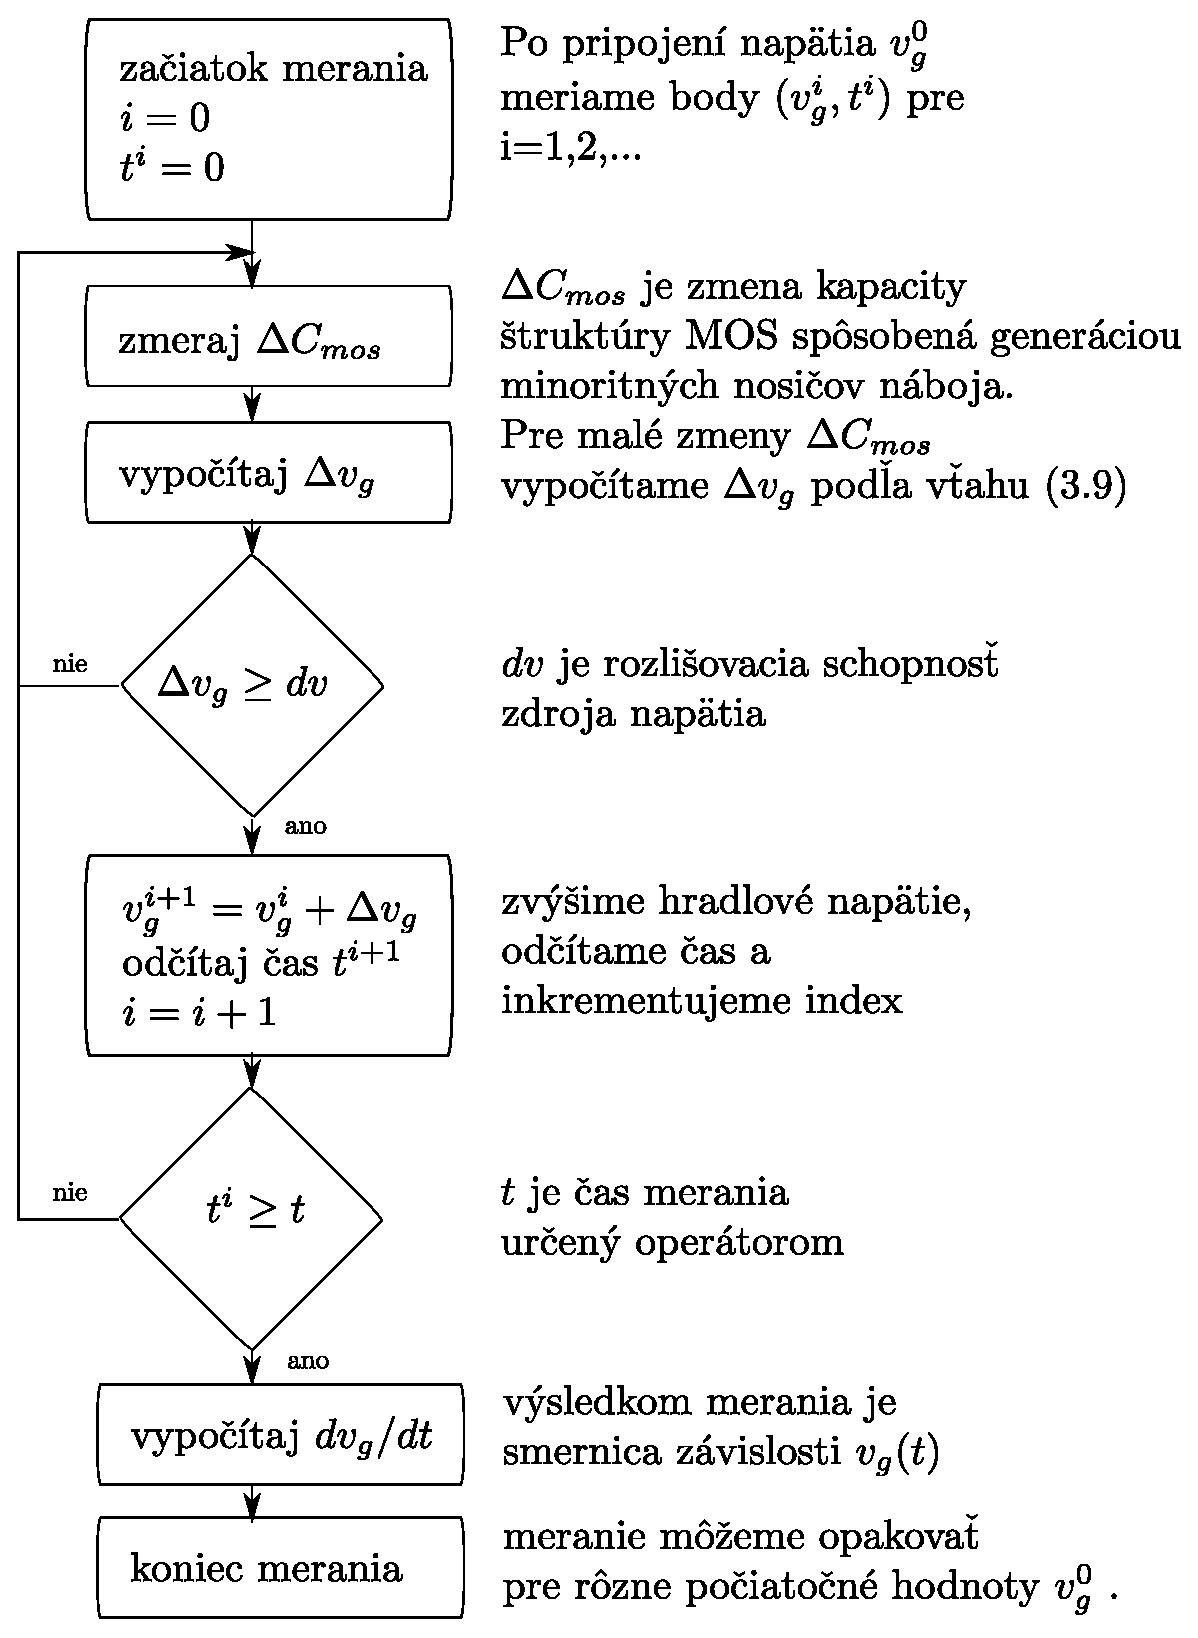
\includegraphics[scale=0.55,keepaspectratio]{Figures/diagram-2.EPS}\label{diagram:2}
\end{diagram}

\begin{figure}[h!]\centering
  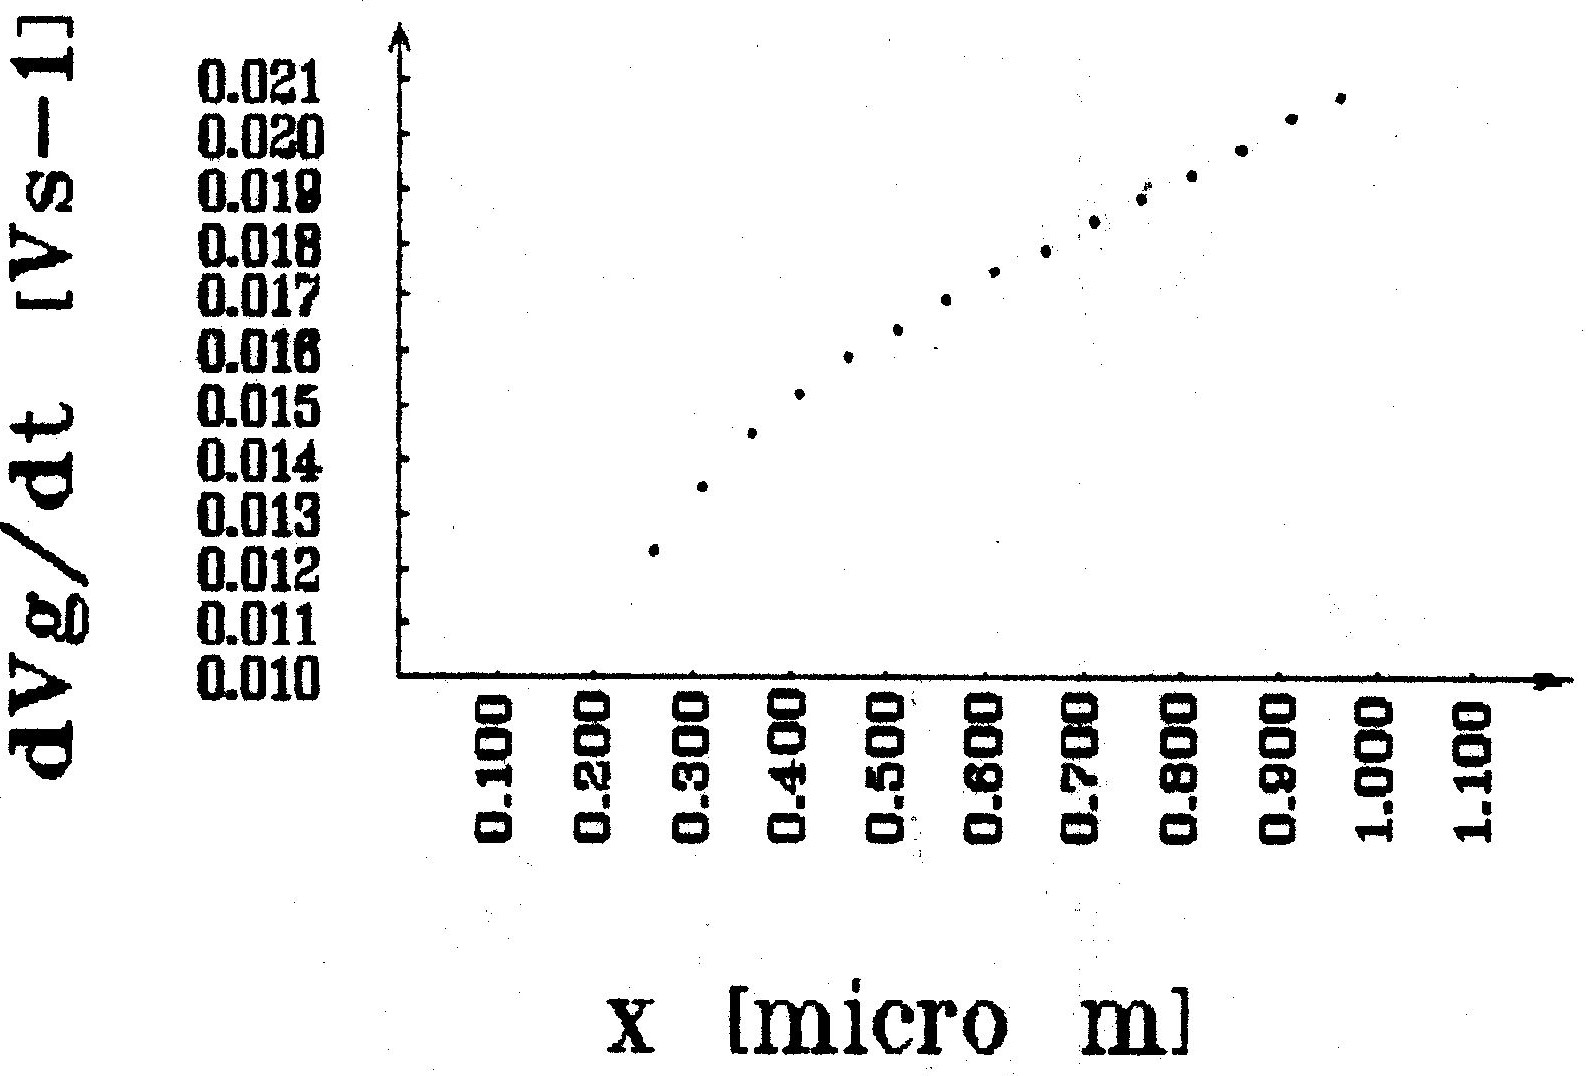
\includegraphics{Figures/fig-3-5.eps}
  \caption[Závislosť $\frac{dV_g}{dt}$ od šírky OPN získaná pomocou
    metódy konštantnej šírky OPN]{Závislosť $\frac{dV_g}{dt}$ od šírky
    OPN získaná pomocou metódy konštantnej šírky OPN.}\label{fig:3.5}
\end{figure}
%OBR19.BIT

Na obrázku~\ref{fig:3.5} je znázornená závislosť $\frac{dV_g}{dt}$ od
šírky OPN\@. Za predpokladu udržania konštantnej šírky OPN sa nemenia
potenciálové pomery v polovodiči a generácia minoritných nosičov je
konštantná, z čoho vyplýva linearita závislosti $V_g(t)$.  Smernice
$\frac{dV_g}{dt}$ potom možno určiť lineárnou regresiou nameraných
závislostí $V_g(t)$. Nie je ťažké si predstaviť, že
vzťahy~\ref{eq:3.6} až~\ref{eq:3.8} predstavujú diskretizáciu
spojitého priebehu $\tau_g(x)$. Ak namerané hodnoty
$\frac{dV_g}{dt}=f(x)$ aproximujeme spojitou funkciou, môžeme vyjadriť
hĺbkový profil $\tau_g(x)$ vzťahom

\begin{equation}\label{eq:3.10}
  \tau_g(x) = \frac{qn_i}{2C_{ox}} {\Bigg[\frac{d\big[\frac{dV_g}{dt}\big]}{dx}\Bigg]}^{-1}
\end{equation}

Na obrázku~\ref{fig:3.6} je znázornený priebeh $\tau_g(x)$, vypočítaný
z nameraných dát zobrazených na obrázku~\ref{fig:3.5} a na
obrázku~\ref{fig:3.7} je hĺbkový koncentračný profil $N(x)$ skúmanej
štruktúry.

\begin{figure}[h!]\centering
  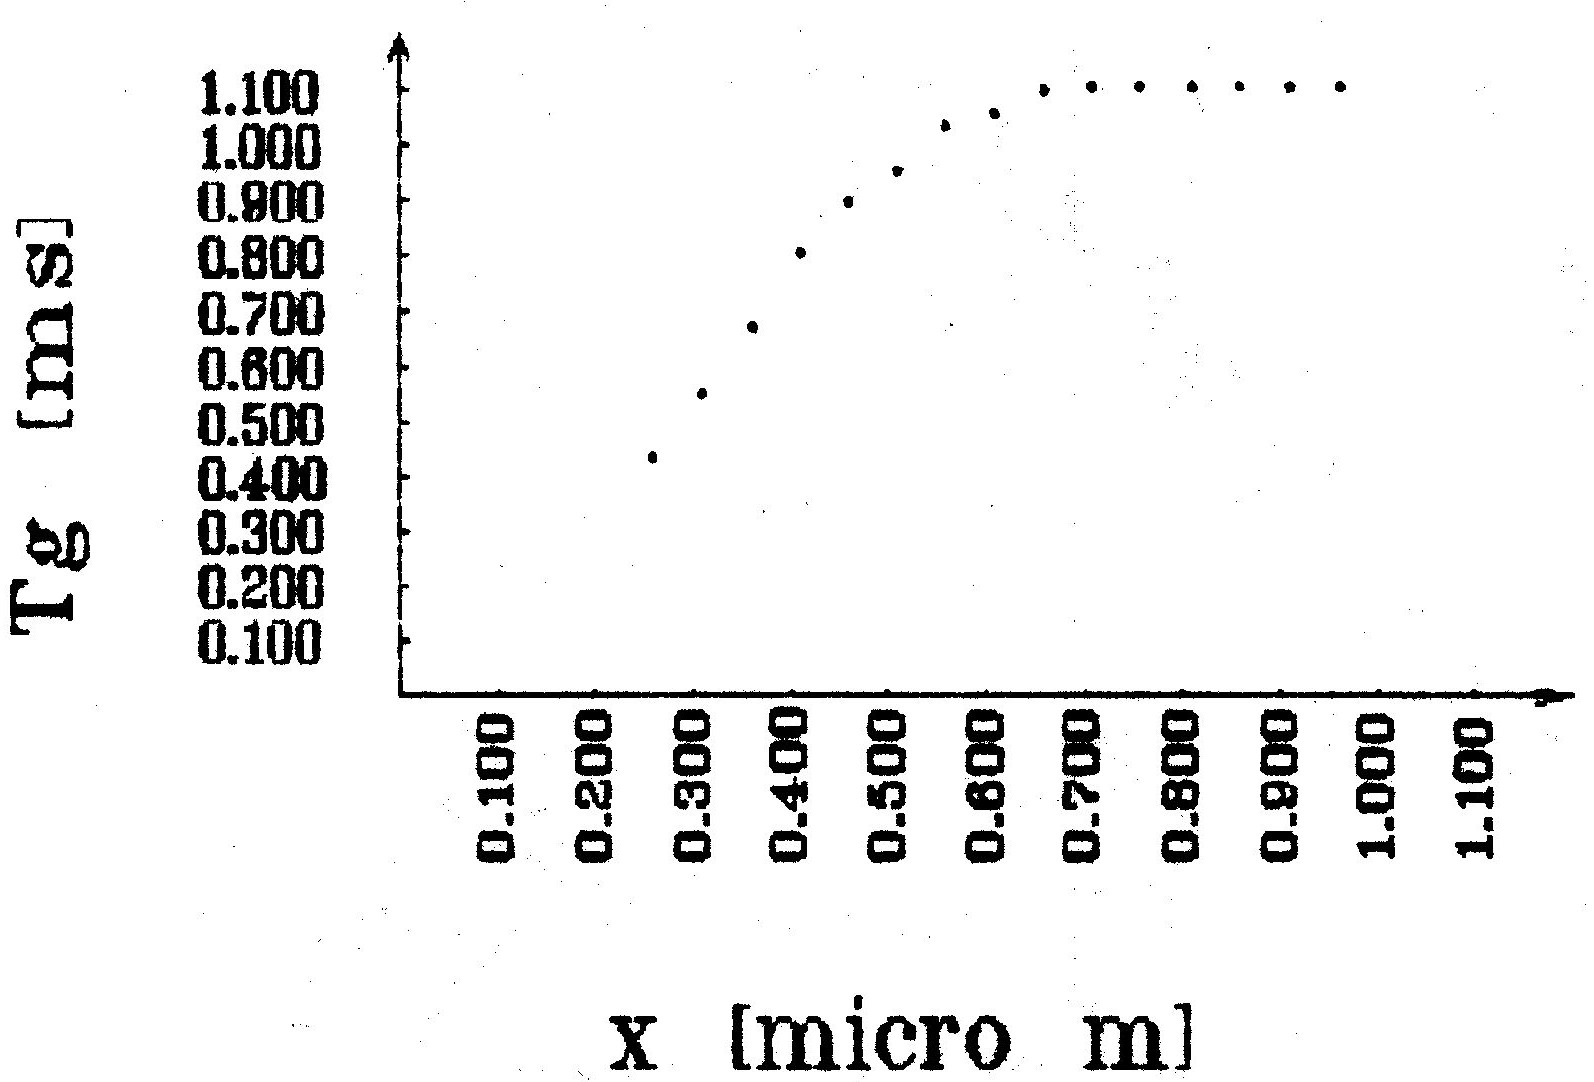
\includegraphics{Figures/fig-3-6.eps}
  \caption[Hĺbkový profil generačného času života minoritných nosičov
  náboja]{Hĺbkový profil generačného času života minoritných nosičov
  náboja.}\label{fig:3.6}
\end{figure}
%OBR20.BIT

\begin{figure}[h!]\centering
  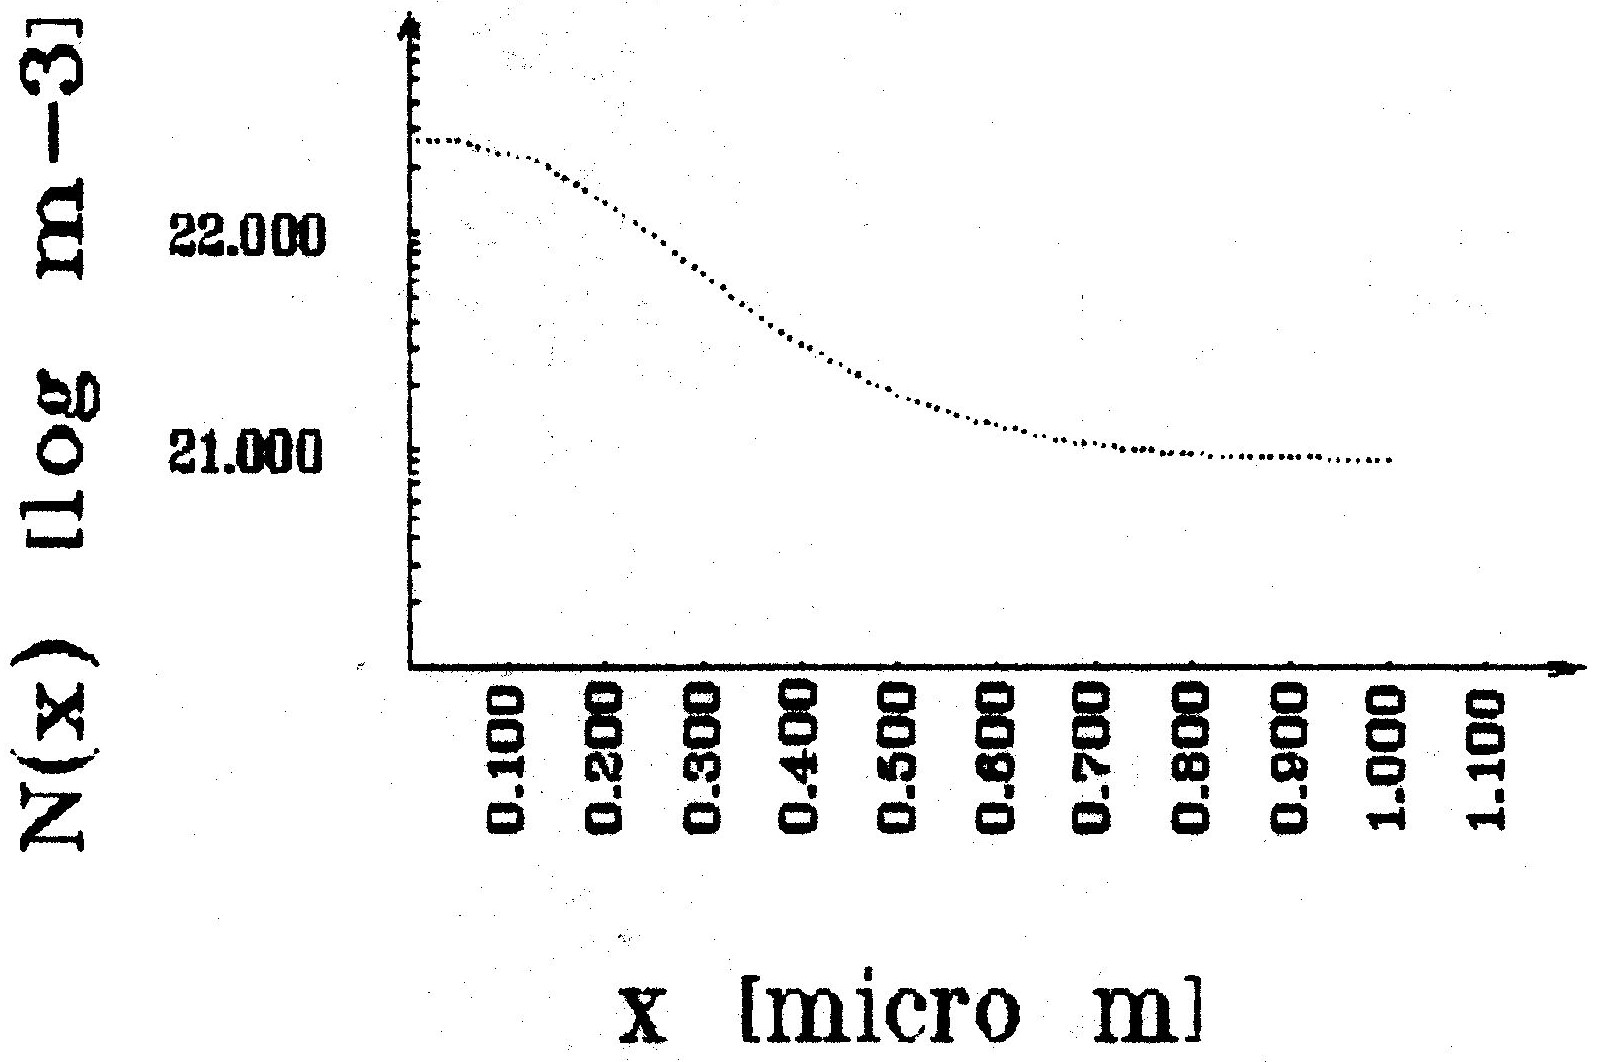
\includegraphics{Figures/fig-3-7.eps}
  \caption[Hĺbkový profil koncentrácie dotujúcich prímesí
  $N(x)$]{Hĺbkový profil koncentrácie dotujúcich prímesí
  $N(x)$. Koncentračný profil prímesí bol vytvorený implantáciou
  $P^{31}$ s dávkou $8.0$ $10^{15}m^{-2}$ pri energii $120 keV$.
  Aktivácia prebiehala počas 40 minút pri teplote $1050 \degree C$ v
  atmosfére $N_2$.}\label{fig:3.7}
\end{figure}
%OBR21.BIT


\begin{thebibliography}{}

\bibitem[3.1]{3.1}
Pierret R.F., Small D.W.: IEEE Trans.\ on elektron.dev. 22 (1975) s.1052.

\bibitem[3.2]{3.2}
Zerbst M.: Z. Angew. Phys. 22 (1966), s.30.

\bibitem[3.3]{3.3}
Eades W.D., Shott J.D., Swanson R.M.: IEEE Trans.\ on elektron.\ dev. 30 (1983) s.1274.

\bibitem[3.4]{3.4}
Nicollian E.H., Brews J.R.: Solid St.\ Electron.  27 (1984) s.953.

\bibitem[3.5]{3.5}
Ziegler K., Klausmann E.: Appl. Phys. Lett. 26 (1975) s.400.

\bibitem[3.6]{3.6}
Boulin D.M., Brews J.R., Nicollian E.H.: Solid St.\ Electron. 27  (1984) s.977.

\bibitem[3.7]{3.7}
Brews J.R., Nicollian E.H.: Solid  St.\ Electron. 27 (1984) s.963.

\bibitem[3.8]{3.8}
Botka V.,Csabay O., Jamrich M.: 5.celoštátna konferencia Mikroelektronika 1989, Dom techniky ČSVTS Bratislava, 1989 s.59.

\bibitem[3.9]{3.9}
Jamrich M.: Q-C metóda pre skúmanie štruktúr MIS\@. Diplomová práca, Katedra mikroelektroniky, EF SVŠT, Bratislava 1988.

\bibitem[3.10]{3.10}
Beyer A., Markgraf W.: Wiss. Z. d. Techn. Hochsch. Karl-Marx-Stadt 28 (1986) s.479.

\bibitem[3.11]{3.11}
Lal, Vasi: Solid St.\ Electron. 30 (1987) s.801.

\bibitem[3.12]{3.12}
Hof, Morthers, Roenker: Solid St.\ Electron. 31 (1988) s.937.

\bibitem[3.13]{3.13}
Pilka K.: Nerovnovážna kapacitná metóda s konštantnou šírkou OPN, Katedra mikroelektroniky, EF SVŠT, Bratislava 1989.

\end{thebibliography}
